\acresetall
\chapter{Learning and Memory}
\label{ch:intro:memory}
Learning and memory define who we are and shape who we will become.
Memory and it's various components -- learning, adaptation, plasticity, association, conditioning -- are fundamental features of nervous systems across all organisms.
The unparalleled ability of humans to learn and adapt to our world is perhaps our greatest genetic adaptation.
Over time, our understanding of memory has evolved from the earliest quantifications of the limits of human memory \citep{Ebbinghaus1885} to a molecular understanding of the changes within the brain that occur following learning \citep{Kandel2001}.

In the following sections I aim to describe an understanding of memory, the brain structures underlying it, and cellular phsyiological correlates of learning relevant to my later studies.
In discussing learning and memory, I will first focus on spatial memory as a core component of episodic memory (\ref{sec:intro:memory:memory}) and how we experimentally study it.
While learning-related changes are fundamental to every neuron in the nervous system, I will primarily focus on the role of the \ac{HPC} in learning and memory, as the \ac{HPC} is most relevant to the memory systems I will be studying (\ref{sec:intro:memory:structure}).
Finally, I will discuss our current understanding of cellular and circuit mechanisms by which the the brain encodes and recalls memory, with a specific emphasis on hippocampal place cells underlying spatial memory (\ref{sec:intro:memory:physiology}).

\section{Memory}






Episodic memory is 
Episodic memory \citep{Tulving1972}
% Ebbinghaus H (1885). Über das Gedachtnis, Dunker & Humbolt.
% https://books.google.com/books?id=kfA0AAAAMAAJ&ots=hjMhksDE3X&dq=Ebbinghaus%20H%20(1885).%20%C3%9Cber%20das%20Gedachtnis%2C&lr&pg=PA1#v=onepage&q&f=false

% \begin{quote}
% Episodic memory retrieves and stores information about temporally dated episodes or events, and temporal-spatial relations among these events. A perceptual event can be stored in the episodic system solely in terms of its perceptible properties or attributes, and it is always stored in terms of its autobiographical reference to the already existing contents of the episodic memory store. The act of retrieval of information from the episodic memory store, in addition to making the retrieved contents accessible to inspection, also serves as a special type input into episodic memory and thus changes the contents of the episodic memory store. The system is probably quite susceptible to transformation and loss of information. While the specific form in which perceptual input is registered into the episodic memory can at times be strongly influenced by information in semantic memory-we refer to the phenomenon as encoding-it is also possible for the episodic system to operate relatively independently of the semantic system.
% \attrib{\citealt[pgs.~385-386]{Tulving1972}}
% \end{quote}

% \begin{quote}
% Consider now a typical memory experiment in which a subject is asked to study and remember a list of familiar words or pair of words. This is an episodic memory task. The occurrence of a verbal item in a given list, at a particular time, and in specific temporal relation to other items in the list is an autobiographical episode having no necessary extra-episodic denotative reference. The subject has successfully retrieved information about this episode when he responds to the retrieval query with the reproduction if an appropriate copy of the input item.
% \attrib{\citealt{Tulving1972}}
% \end{quote}

% \begin{quote}
% Each experienced event always occurs at a particular spatial location and in a particular temporal relation to other events that already have occurred, events occurring simultaneously with it, or events that have not yet occurred. These temporal relations among experienced events are also somehow represented as properties of items in the episodic memory system. To ask a person about some item in episodic memory means to ask them when did event $E$ happen, or what events happened at time $T$. Retrieval of information of this kind from episodic memory is successful if the person can describe the perceptible properties of the event in question and more or less accurately specify its temporal relations to other events. Temporal coordinates of an event and its representation in episodic memory of course need not be specified in terms of the clock and the calendar. They could be recorded in terms of temporal occurrences of other events in some as yet little understood manner.
% \attrib{\citealt[pg.~388]{Tulving1972}}
% \end{quote}

Eichenbaum H, Yonelinas AR, Ranganath C (2007): The medial tempo- ral lobe and recognition memory. Annu Rev Neurosci 30:123–152.
Milner B, Squire LR, Kandel ER (1998): Cognitive neuroscience and the study of memory. Neuron 20:445–468.
23.
Fortin NJ, Wright SP, Eichenbaum H (2004): Recollection-like memory retrieval in rats is dependent on the hippocampus. Nature 431:188– 191.
Sauvage MM, Fortin NJ, Owens CB, Yonelinas AP, Eichenbaum H (2008): Recognition memory: Opposite effects of hippocampal dam- age on recollection and familiarity. Nat Neurosci 11:16–18.

\subsection{Spatial memory}\label{sec:intro:memory:spatial}
Spatial memory is the aspect of our memory that instills our sense of direction and allows us to know where we are at any given time (our personal `GPS'), imagine or plan where we will be in the future, and know where we were when we recall particular memories.
Spatial navigation consists of two primary components: location relative to an allocentric map of the world, and egocentric update cues arising from orientation (\textsc{head direction cells}) and other vestibular input.
The dominance of alocentric or egocentric navigation depends upon the precise nature of the environment being explored; egocentric dominates in cue-rich environments, while alocentric navigation dominates when landmarks are lacking or in the dark \citep{Knierim1998}.

Spatial memory has been studied extensively in rodents, in large part because it a well-defined and tractable area of research.
As rodents can not be asked to recall past events, we need assays that can probe for evidence of these memories (\nameref{sec:intro:memory:spatial-reward}).
Not only do we have good behavioral tests for spatial memory in rodents, but we have identified the cognitive map of the memory itself (\nameref{ec:intro:memory:place_cells}).
% Allocentric navigation in particular is \ac{HPC}-dependent \citep{OKeefe1978, Smith1989}, not egocentric.

\subsubsection{Spatial memory as episodic memory}\label{sec:intro:memory:spatial-episodic}
In 1972 Endel Tulving coined the term \textsc{episodic memory}, describing it as follows:

\begin{quote}
Episodic memory retrieves and stores information about temporally dated episodes or events, and temporal-spatial relations among these events...Each experienced event always occurs at a particular spatial location and in a particular temporal relation to other events that already have occurred, events occurring simultaneously with it, or events that have not yet occurred.
\attrib{\citealt{Tulving1972}}
\end{quote}

As this interpretation suggests, the specific of the events itself are inseparable from the time at which it occurred and the location of the event (or individual aspects of the event).
This is most obvious in autobiographical episodic memory, where experiences (e.g. waiting in line to get lunch) are remembered along with the location (e.g. Mike's Bagels at 168\super{th} and Broadway) and the time (e.g. last Tuesday around 2PM) they occurred.
This applies to psychological memory tests as well, such as remembering words on a list, where the temporal order of items on the list (I saw `orange' before `banana') and the visio-spatial arrangement of the words on the paper list (`boat' was written above `car') are core components of the stored memory.
Even more than being a component of episodic memory, spatial memory may in fact \emph{be} episodic memory.
The brain structure most closely associated with episodic memory (\nameref{sec:intro:memory:hpc}) has also shown to contain cells which directly map to real world locations (\nameref{sec:intro:memory:place_cells}).
Indeed it has been proposed that the same neural mechanisms may underly both the ability to store the relationship amongst objects in a remembered experience, and the relationship between landmarks contributing to a map of space \citep{Buzsaki2013}.

\subsection{Spatial reward learning}\label{sec:intro:memory:spatial-reward}
Tests of spatial memory are fundamental tools for rodent researchers.
The most widely used assay of spatial memory is the \textsc{Morris water maze} \citep{Morris1984}.
While there is variability in the details of the protocol, the general structure is usually the same.
Briefly, the `maze' is a large water-filled tub with a single hidden platform under the surface of the water.
Mice or rats are placed in the maze and over successive trials eventually learn to use distal cues around the room to locate the platform.
Probe trials generally consist of removing the platform and scoring the fraction of time spent in the correct quadrant as a measure of spatial memory.
More recently, virtual reality variations of the Morris water maze have been developed that allow for head-fixed spatial learning tasks in rodents \citep{Aronov2014} or the ability to mirror rodent experimental paradigms in humans \citep{}.

One particular variation is the annular water maze used by \citeauthor{Hollup2001a}, which adds an inner wall to the large circular pool creating a `one-dimensional' circular track that the mice swim around.
This task is similar to the goal-oriented learning task (\autoref{sec:intro:techniques:GOL}) that I use throughout my primary experiments; both tasks require rodents to find hidden rewards in a simplified `one-dimensional' environment while recording from hippocampal area CA1 pyramidal cells and quantify both the task performance and place cell enrichment of the reward location.
In particular, the authors find an accumulation of place cells around the escape platform (\autoref{fig:intro:memory:hollup}), a finding which I replicate and expand upon in my GOL task (\autoref{sec:df:results:enrichment}). 
\begin{figure}
	\centering
	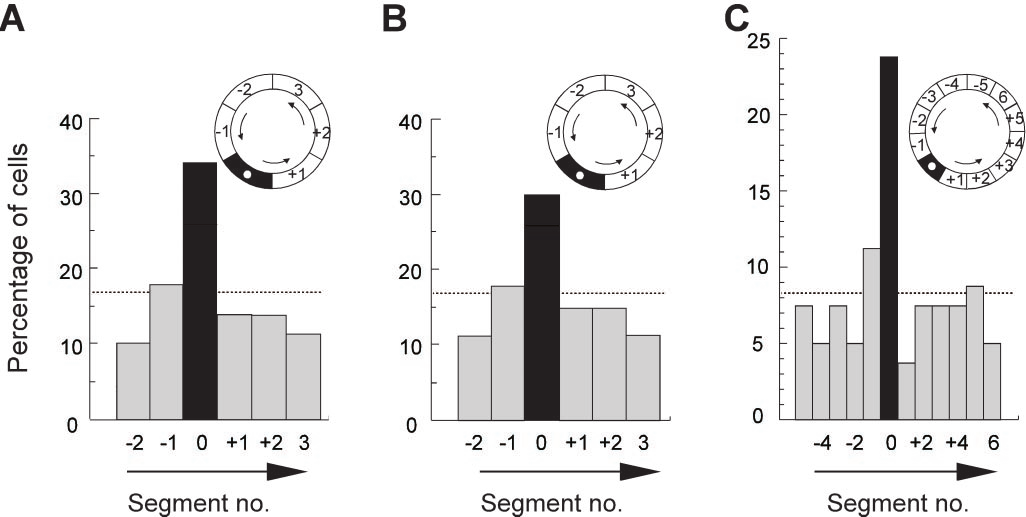
\includegraphics[width=0.7\textwidth]{intro/Hollup_accumulation}
	\caption[Distribution of firing fields from Hollup et al.]{Distribution of firing fields after training with a constant platform location.
	(A) Percentage of firing fields in each 60$^{\circ}$ segment of the corridor (80 cells; average of 3 probe tests). Field location was defined as the segment with the maximal averaged firing rate. Firing fields accumulated in the platform segment (segment 0, black). The chance level was at 16.7\%. Inset, Diagram of the corridor. Arrows indicate swim direction.
	(B) Percentage of firing fields in each 60$^{\circ}$ segment after directional sorting (same trials and same symbols as described in A). Only data sampled during swimming in the preferred direction are retained.
	(C) Percentage of firing fields in segments of 30$^{\circ}$ after directional sorting. The platform was in the middle of segment 0.
	Reproduced from \citet{Hollup2001a}.}
	\label{fig:intro:memory:hollup}
\end{figure}

Conceptually similar, but drier, are the Barnes or cheeseboard maze \citep{Barnes1979}\citep{Kesner1991}\citep{Dupret2010a}.
These mazes are consist of a large platform with holes throughout.
These holes can either be escapes for the mice/rats to avoid the exposure of the platform, or baited/rewarded.
Either way, the degree of learning can be quantified by latency to finding the correct location or time spent near previously rewarded locations during un-rewarded probe trials.
In a study by \citeauthor{Dupret2010a} which partially inspired my own work, the authors used a cheeseboard maze to examine hippocampal functional correlates of learning and memory (see \nameref{sec:df:methods:comp}).
They authors identified an increase in the fraction of hippocampal area CA1 place cells that encoded the reward location, the magnitude of which correlated with task performance (\autoref{fig:intro:memory:dupret}a,b).
In addition they found properties of sharp-wave ripples (SWRs) that also correlated with task performance -- the fraction of pyramidal cells that participated in sharp-wave ripple events during exploration (eSWRs) and the similarity of the pyramidal cell firing patterns during off-line SWRs (sSWRs) with on-line exploration of the reward locations (\autoref{fig:intro:memory:dupret}c,d).
In light of evidence pointing to a central role for SWRs in long-term memory consolidation \citep{Buzsaki2015}, it's tempting to interpret these findings as task performance being aided by an increased number of pyramidal cells encoding a memory of the reward locations during exploration and increased `remembering' of the rewarded locations during sleep.

\begin{figure}
	\centering
	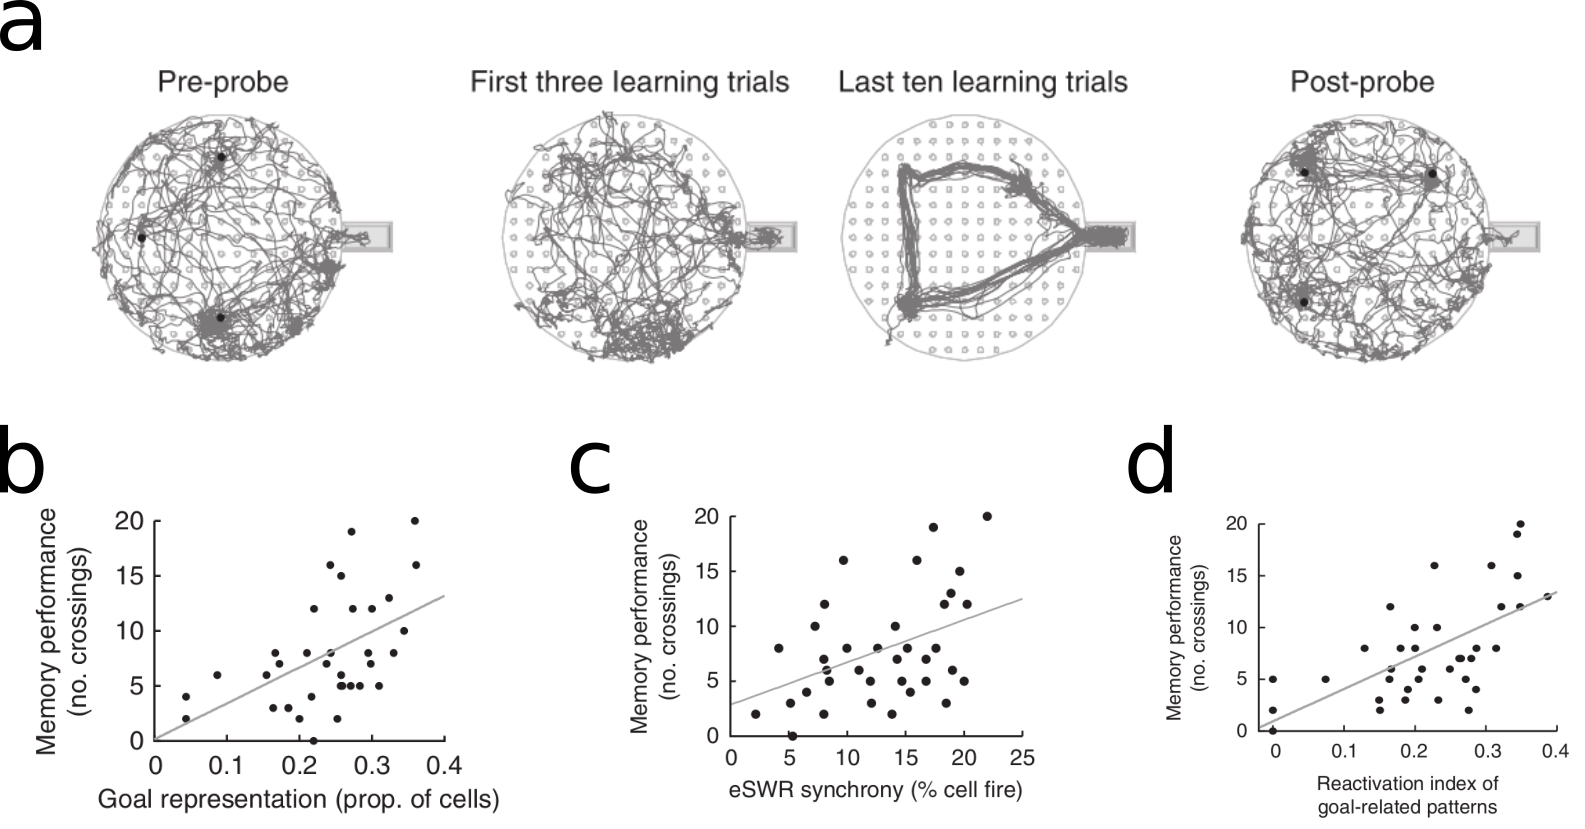
\includegraphics[width=0.7\textwidth]{intro/Dupret_cheeseboard_and_correlates}
	\caption[Cheeseboard task and behavioral correlates from Dupret et al.]{Cheeseboard task and behavioral correlates from Dupret et al.
	(a) Representative examples of an animal's path; for clarity, only the first 10 min of each probe session is depicted (black dots, learnt goal locations).
	(b) Scatter plot showing post-probe memory performance (number of crossings) as a function of the proportion of CA1 place cells at goal location during the end of learning (gray: regression line, r = 0.511, P=0.0014).
	(c) Scatter plot showing post-probe memory performance (number of crossings) as a function of `eSWR synchrony' (percentage of CA1 pyramidal cells that fire in eSWR) at the end of learning (gray: regression line, r = 0.418, P=0.011).
	(d) Scatter plot showing post-probe memory performance (number of crossings at a given goal location) as a function of the proportion of sSWRs in which assembly patterns represented the same goal location (gray: regression line, r = 0.620, P=0.00005)
	Figures rearranged and reproduced from \citet{Dupret2010a}.}
	\label{fig:intro:memory:dupret}
\end{figure}


\section{Memory in the brain}\label{sec:intro:memory:structure}
\todo{Expand more generally on brain regions involved in memory}

\subsection{The Hippocampus}\label{sec:intro:memory:hpc}
While `learning' in it's broadest sense is a fundamental feature of every neuron, in mammals, the \ac{HPC} is central to the formation, storage, and recall of explicit memories of experiences.
The \ac{HPC} has been central to our study of memory at least since Scoville and Milner first reported in the 1950's on Henry Molaison (patient H.M.) who had profound anterograde amnesia following the bilateral removal of large portions of the medial temporal lobes, which includes the \ac{HPC} and parahippocampal structures \citep{Scoville1957}.
\todo{Expand on patient HM}
Since then, numerous studies have shown that the \ac{HPC} is essential for normal formation and recall of long term episodic and semantic memory \citep[reviewd in][]{Eichenbaum2000, Burgess2002}.

The hippocampal is one of the best characterized neuronal circuits within the mammalian brain.
The principal neurons in the \ac{HPC} communicate through the classically-defined trisynaptic loop: perforant path fibers project from the entorhinal cortex (EC) to granule cells in the dentate gyrus, which in turn send mossy fiber projections to CA3 that finally travel along the Schaffer collateral pathway and synapse upon proximal apical and basal dendrites of CA1 pyramidal cells (CA1PCs).
CA1PCs then send processed information to cortical and subcortical areas, including return projections back to deep layers of EC.

Finally, both principal neurons and GABAergic interneurons are targeted by afferents from neuromodulatory nuclei, including cholinergic and GABAergic projections from the medial septum  \citep{Klausberger2008}, serotonergic and glutamatergic projections from the raphe nuclei \citep{Varga2009}, as well as dopaminergic and noradrenergic projections from the ventral tegmental area \citep{Gasbarri1997} and locus coeruleus \citep{Foote1983}.


Burwell RD (2000): The parahippocampal region: Corticocortical connectivity. Ann N Y Acad Sci 911:25–42.
\subsection{CA1}
\begin{figure}
	\centering
	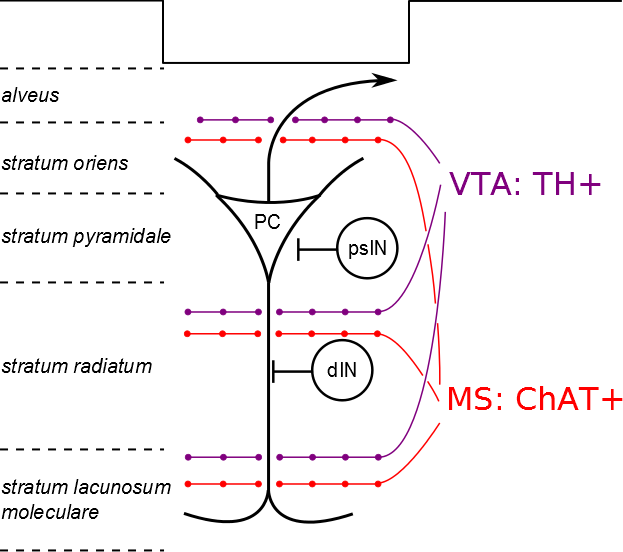
\includegraphics[width=0.5\textwidth]{intro/CA1-schematic_INs_VTA_MS}
	\caption{Schematic of major inputs to CA1 pyramidal cells}
	\label{fig:intro:memory:CA1_schematic}
\end{figure}


\subsection{Other}
In discussing the role of the \ac{HPC}, I've focused on spatial memory, but this is clearly not the sole role of the \ac{HPC}.
Social
Time
conversion to longterm memory
environment
pattern completion/separation

\section{Functional correlates of memory}\label{sec:intro:memory:physiology}

\subsection{Memory engrams}

\subsection{Spatial maps}
Perhaps the best-studied 
Throughout the \ac{HPC} (dentate gyrus, CA3, CA2, and CA1) there are principal cells that fire selectively at specific locations within an environment (\textsc{place cells}).
Our understanding of place cells is a uniquely well-characterized functional mapping of the real world multiple synapses from both sensory and motor cortices.

Within the entorhinal coretx, principal cells take on a variety of spatial firing properties, but one of the main categories are cells that fire at regularly spaced intervals throughout an environment (\textsc{grid cells}).
Place cells and grid cells together form the cellular foundation for the mammalian navigation system, and their discovery was recently awarded with the Nobel Prize in Medicine.
Pyramidal cells in hippocampal area CA1 are the principal excitatory neuron in that region and the primary output from the \ac{HPC}.
As an animal explores an environment these pyramidal cells show sparse spatially-modulated changes in firing rates (place cells) that are established rapidly and subsequently remain stable \citep{O'Keefe1971}\citep{Frank2004}.
These place cells form an allocentric map of the environment, which is essential for normal episodic memory function \citep{Smith2006c}\citep{Nakazawa2004}\citep{Buzsaki2013}.

\subsection{Place cells}\label{sec:intro:memory:place_cells}
\begin{figure}
	\centering
	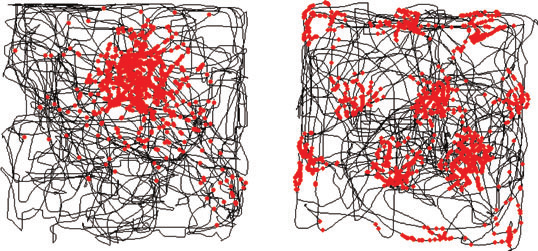
\includegraphics[width=0.7\textwidth]{intro/Moser_2008_place_grid}
	\caption[Place cell in the hippocampus and grid cell in the MEC]{Place cell in the hippocampus (a) and grid cell in the medial entorhinal cortex (MEC) (b).
	Spike locations (\emph{red}) are superimposed on the animal’s trajectory in the recording enclosure (\emph{black}).
	Whereas most place cells have a single firing location, the firing fields of a grid cell form a periodic triangular matrix tiling the entire environment available to the animal.
	Reproduced from \citet{Moser2008}.}
	\label{fig:intro:memory:place_grid}
\end{figure}

\subsubsection{Remapping}
\citep{Muller1987}
Place cells, like other forms of memory, are constantly trying to balance two competing constraints: on the one hand, their firing needs to be stable in order to be a helpful representation of the environment, but on the other hand, their firing needs to be plastic enough to constantly encode new environments, forget irrelevant information, and adapt to new features.
Place cells changing their firing properties to incorporate new features of the world is known as \textsc{remapping}.
A given place cell is defined by it's spatial tuning -- it's place field -- and it's firing rate gain with the place field.
These seem to be independent factors, as either can remap separately.
\textsc{Global remapping} is the collective remapping of place field locations across a population of place cells.
Alternatively, \textsc{rate remapping} is a change in place field gain (the ratio of firing rate in to out of the place field), while place fields locations remain fixed.
While place field location and firing rate gain remap separately....\textsc{partial remapping}.
\todo{Include Kentros}